% vim: set tw=0:
\documentclass{beamer}
\usepackage{graphicx}
\usepackage{booktabs}

% Reasonable themes:
% Antibes Bergen Berkeley Berlin Frankfurt Goettingen Ilmenau Luebeck Malmoe
% Montpellier PaloAlto Rochester Singapore Szeged Warsaw bars boxes
% compatibility default lined plain shadow sidebar split tree
% And these ones include the author's name on every slide:
% Berkeley

% Declare themes.
\mode<presentation>
\usetheme{UWHEP}

% Personal macros.
\newcommand{\email}[1]{{\texttt #1}}
\newcommand{\newframe}[1]{\section{#1}
    \frametitle{\sc{#1}}}
\newcommand{\subframe}[1]{\subsection{#1}
    \frametitle{\sc{#1}}}
\newcommand{\supers}[1]{\ensuremath{^\textrm{#1}}}
\newcommand{\subs}[1]{\ensuremath{_\textrm{#1}}}
\newcommand{\ca}{\ensuremath{\sim}}

% Author information.
\title{Site report: Wisconsin}
\author[Maier, Mohapatra]{
    Will Maier \and Ajit Mohapatra\\ 
    {\tt wcmaier@hep.wisc.edu}\\
    {\tt ajit@hep.wisc.edu}}
\institute[Wisconsin]{University of Wisconsin - High Energy Physics}
\date[2008.04.11]{USCMS T2 Workshop - Purdue, 2008.04.11}
\logo{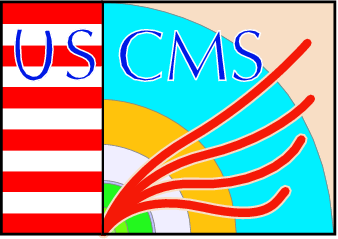
\includegraphics[height=0.6cm]{../../../Graphics/USCMS_logo.png}\hspace{.1cm}
\includegraphics[height=0.75cm]{../../../Graphics/UW_logo.png}}

\begin{document}

% Notes:
%Guidelines for site reports:  What are your plans for completing
%hardware deployment in 2008?  Describe site commissioning status,
%and your experience in getting there.  Describe what expectations
%you think your local or regional community has of you.
%
%OTHER:
%    * condor upgrades
%
%* Hardware commissioning (now vs future)
%    * KSI2K (nodes, CPUs)
%    * TB dCache (disk)
%    * Network (wires)
%    * Site (HVAC)
%* Site commissioning status/experience (what've we done to improve)
%    * SAM
%        * stageout: dCache
%            * aggressive replication policy
%            * new server hardware (PNFS, etc)
%            * new monitoring
%            * debugging
%        * software installation
%            * rerouted CMSSW install jobs to dedicated slots
%
%    * JR
%        * Correct advertisement to RB/DBS (via DBII)
%        * Presence of datasamples
%        * Jobs function (condor, dcache r/w?)
%    * PhEDEx
%        * Links
%* Regional/local community expectations
%    * HLT validation (incl .eu physicists)
%    * Local students (4x) running jobs: Photon jets, Electroweak,
%      QCD


\begin{frame}
    \titlepage
\end{frame}

\section{Overview}
\begin{frame}
    \tableofcontents
\end{frame}

\section{2008 Hardware Deployment}
\subsection{Storage}
\begin{frame}
\begin{itemize}
    \item Through 2007 - 2008, purchased 500 GB - 750 GB SATA disks
    \item Added disk to integrated UW Plasma cluster
    \item No plans for more dedicated storage
    \item May 2008: 128 TB on 32 1U servers (1 TB SATA disks)
\end{itemize}

\begin{columns}
\column{2.5in}
\begin{table}
    \begin{tabular}{lr}
        \toprule
        Dedicated dCache & 45 TB \\
        dCache + Condor & 78 TB \\
        \midrule
        Raw & 123 TB \\
        Replicated & 80 TB \\
        \bottomrule
    \end{tabular}
    \caption{2007 Storage Status}
    \label{2007_storage_status}
\end{table}

\column{2.5in}
\begin{table}
    \begin{tabular}{lr}
        \toprule
        Dedicated dCache & 45 TB \\
        dCache + Condor & 175 TB \\
        \midrule
        Raw & 220 TB \\
        Replicated & 110 TB \\
        \bottomrule
    \end{tabular}
    \caption{2008 Storage Status}
    \label{2008_storage_status}
\end{table}

\end{columns}
\end{frame}

\subsection{Compute Resources}
\begin{frame}
\begin{itemize}
    \item During 2007, all compute nodes upgraded to SL4
    \item Integrated 24 UW Plasma nodes, 32 new dual/quad Xeons
    \item High priority, opportunistic access to more than 2k GLOW CPUs
    \item May 2008: 256 CPUs @ 3.0 GHz Xeon on 32 1U servers
\end{itemize}
\begin{columns}
\column{2.5in}
\begin{table}
    \begin{tabular}{lr}
        \toprule
        CPU Class           & KSI2K \\
        \midrule
        2 x 2.4 GHz Xeon    & 64.80 \\    % g3
        2 x 2.8 GHz Xeon    & 158.6 \\    % g4, g5, g6
        2 x 3.0 GHz Xeon    & 99.2 \\     % g7, g8
        4 x 1.8 GHz Opteron & 207.0 \\    % g9 (g10 still Plasma)
        \midrule
        Total & 529.6 \\
        \bottomrule
    \end{tabular}
    \caption{2007 Batch Status}
    \label{2007_Batch_status}
\end{table}

\column{2.5in}
\begin{table}
    \begin{tabular}{lr}
        \toprule
        CPU Class           & KSI2K \\
        \midrule
        2 x 2.4 GHz Xeon    & 64.80 \\    % g3
        2 x 2.8 GHz Xeon    & 158.6 \\    % g4, g5, g6
        2 x 3.0 GHz Xeon    & 99.2 \\     % g7, g8
        4 x 1.8 GHz Opteron & 317.0 \\    % g9, g10
        8 x 3.0 GHz Xeon        & 691.2 \\    % g12
        \midrule
        Total & 1330.80 \\
        \bottomrule
    \end{tabular}
    \caption{2008 Batch Status}
    \label{2008_Batch_status}
\end{table}
\end{columns}
\end{frame}

\subsection{Network, Infrastructure}
\begin{frame}
\begin{figure}
    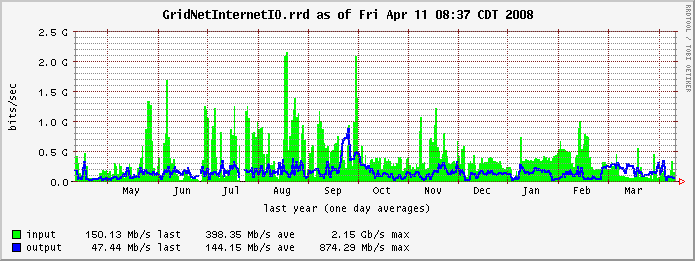
\includegraphics[height=3.5cm]{Graphics/gridnetio-1year.png}
    \caption{Cluster network, April 2007 - April 2008}
\end{figure}

\begin{itemize}
    \item Transfer maxima (in/out):
    \begin{itemize}
        \item Daily averages: 2.15 Gbps/0.8 Gbps
        \item Peak: 5.0 Gbps (in)
    \end{itemize}
    \item Core CMS servers and networking moved to UPS
\end{itemize}
\end{frame}

\subsection{Summary of Status}
\begin{frame}
\begin{itemize}
    \item Currently, Wisconsin exceeds pledge amounts in terms of raw resources
    \item May 2008 purchase will bring replicated storage close to 200 TB
    \item Considering further 'dedicated' storage purchases (Thumper?)
\end{itemize}
\begin{table}
     \begin{tabular}{lrrr}
         \toprule
         Category    & Current       & May 2008      & Pledge Percent \\
         \midrule
         Storage     & 110 TB        & 175 TB        & 87.5\%\footnotemark[1] \\
         CPU         & 1.3 MSI2K     & $\geq$ 2.0 MSI2K & $\geq$ 200\% \\
         \bottomrule
     \end{tabular}
     \caption{Wisconsin pledge status today and in May 2008}
\end{table}

\footnotetext[1]{Aggressively replicated data (ratio: 2.0); 350 TB raw}
\end{frame}

\section{Site Commissioning}
\subsection{Local Effort}
\begin{frame}
\begin{itemize}
    \item Improved dCache replication with PFM has led to fewer transfer/stageout failures
    \item New (64 bit) hardware for core dCache servers (including PNFS) has increased performance 6x - 10x
    \item Rerouted CMSSW installation jobs to better, dedicated hardware to reduce failure rate
    \item Six links commissioned:
    \begin{itemize}
        \item FNAL, CERN, FZK, CNAF, RAL, PIC, IN2P3
    \end{itemize}
    \item Improved Condor scaling
    \begin{itemize}
        \item Removed bottlenecks for job submission
        \item Created {\tt farmout} family of submission scripts for local CMSSW analysis
    \end{itemize}
    \item Developed threading and other performance improvements for PFM
    \begin{itemize}
        \item Replication is critical to Wisconsin storage model
        \item With $>$ 200k files in PNFS namespace and $>$ 330 pools, slow operations drastically reduce PFM performance
    \end{itemize}
\end{itemize}
\end{frame}

\subsection{Recent SAM}
\begin{frame}
\begin{figure}
    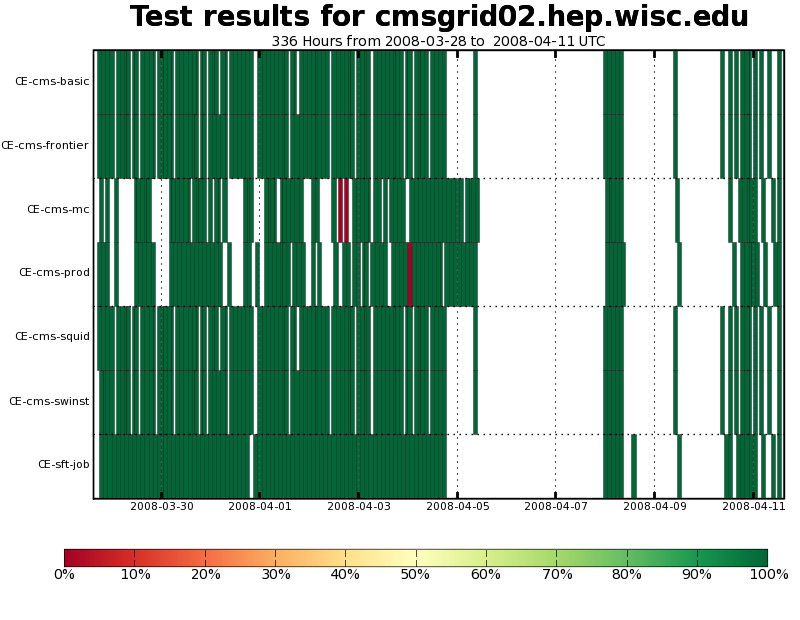
\includegraphics[height=7cm]{Graphics/sam.png}
    \caption{SAM results at Wisconsin - last two weeks}
\end{figure}
\end{frame}

\subsection{Wishlist}
\begin{frame}
\begin{itemize}
    \item More pretty graphing utilities (ideally all in one place)
    \item REST/XMLRPC/other API for direct access to data
    \begin{itemize}
        \item Allows for more robust local (automated) checks
        \item Less work (fewer custom views, etc) for central monitoring folks
    \end{itemize}
    \item Increased collaboration on administration tools
    \begin{itemize}
        \item Excellent start with OSG Storage toolkit
        \item Several parallel efforts at the sites
        \item Shared repository (similar to PhEDEx configs)?
    \end{itemize}
\end{itemize}
\end{frame}

\section{Community Support}
\subsection{HLT Validation and Local Analysis}
\begin{frame}
\begin{itemize}
    \item Several dozen collaborators working on HLT validation
    \item Local students focusing on:
    \begin{itemize}
        \item Photon jets
        \item Electroweak
        \item QCD
    \end{itemize}
    \item Local work is correctly represented on the dashboard
    \begin{itemize}
        \item Users use {\tt farmout} scripts\footnotemark[1] (Dan Bradley)
        \item Script automatically submits jobs for an input dataset based on DBS info and data in local dCache storage
        \item Makes local analysis very convenient
        \item We don't mind providing local user accounts for this sort of successful user analysis
        \item \ca{} 30 active users
    \end{itemize}
\end{itemize}
\footnotetext[1]{http://www.hep.wisc.edu/cms/comp/AnalyzingManyEvents.html}
\end{frame}

\begin{frame}
\begin{figure}
    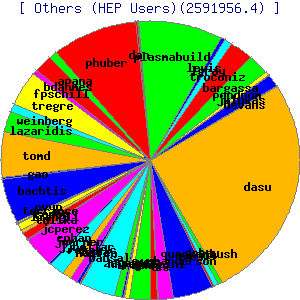
\includegraphics[height=6cm]{Graphics/glow-userpie.png}
    \caption{Cluster users by CPU hours: 2005.10.05 to today ($>$ 2.5M hours)}
\end{figure}
\end{frame}

\end{document}
